\documentclass[aspectratio=169]{beamer}

\usepackage{tikzducks}

\setbeamertemplate{navigation symbols}{}
\setbeamertemplate{background canvas}{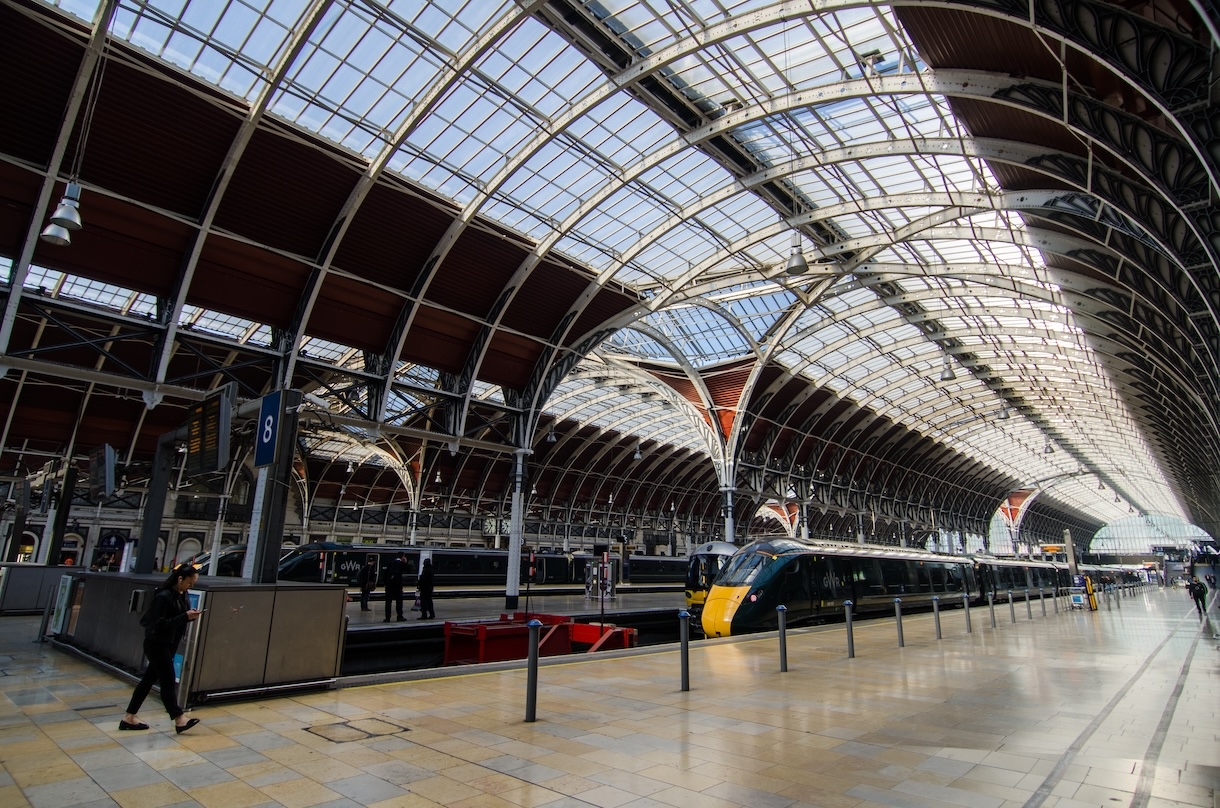
\includegraphics[width=\paperwidth]{Paddington_Station_GWR}}
\graphicspath{{include/}}

% trick taken from https://topanswers.xyz/tex?q=1989
\tikzset{
    use page relative coordinates/.style={
        shift={(current page.south west)},
        x={(current page.south east)},
        y={(current page.north west)}
    },
}

\begin{document}

\begin{frame}
  \begin{tikzpicture}[remember picture, overlay,use page relative coordinates]
    
%    \node[anchor=west,xshift=-\insertoverlaynumber*0.05cm] at (0,0.25) {\scalebox{-1}[1]{
\includegraphics[height=3cm]{ducks}}};
%    \draw[line width=0.5cm,black!70!white] (0.1,0.6) -- ++ (0,-10cm);  
%    \node[inner sep=0pt] at (0.1,0.6) {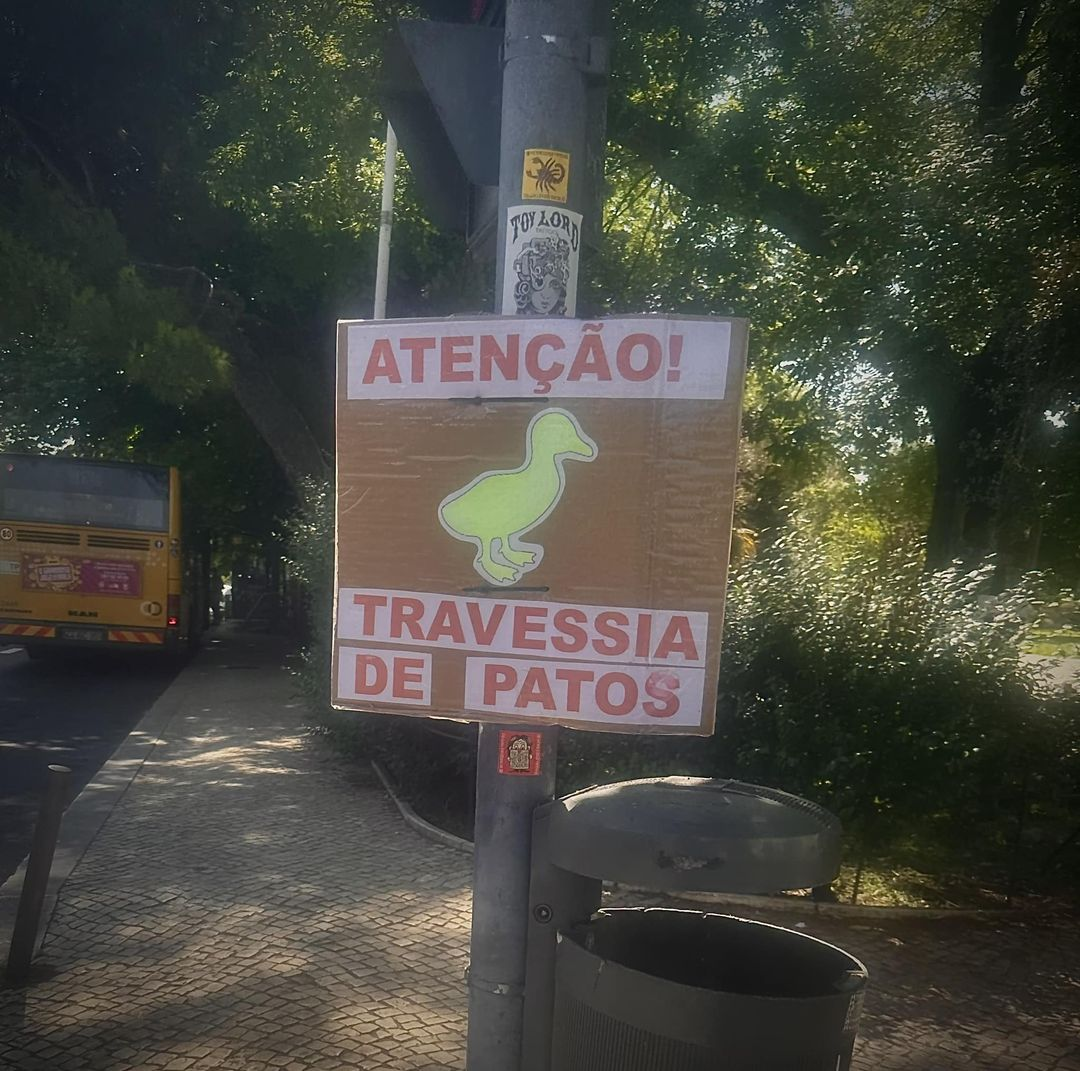
\includegraphics[width=3cm]{patocrossing}};

    % credit for background image
    \node[white,text width=.9\paperwidth,font=\tiny,align=center] at ([yshift=0.35cm]current page.south) {Image by @Jeff Hitchcock \href{https://creativecommons.org/licenses/by/2.0/deed.en}{CC BY 2.0} 
    (\url{https://en.wikipedia.org/wiki/File:Paddington_Station_GWR.jpg})
    };

  \end{tikzpicture}
%  \pause[600]
\end{frame}

\end{document}